\documentclass[9pt]{template/developercv}
\usepackage[danish]{babel}

% Commands
\newcommand{\nametitlebox}[1]{\colorbox{white}{{\Huge\textcolor{black}{\textbf{\MakeUppercase{#1}}}}}}
\newcommand{\link}[2]{\faLink~\href{#1}{\textbf{#2}}}

% Settings
\setlength{\tabcolsep}{2pt}
%----------------------------------------------------------------------------------------
% CUSTOM STRUT FOR EMPTY BOXES
%----------------------------------------- -----------------------------------------------
%\newcommand{\mystrut}{\rule[-.3\baselineskip]{0pt}{\baselineskip}}
\begin{document}

% HEADER (name, contact information)
% ------------------------------------------------------------------------------
% HEADER (name, contact information)
% ------------------------------------------------------------------------------
\begin{minipage}[c]{0.7\textwidth}
  \vspace{-\baselineskip}
  \nametitlebox{Artur Iablokov}{  \huge \faLaptop\ Software Engineer}
  \vspace{1em}

    I am a software engineer with 8 years of experience in payment services and energy
monitoring systems. My curiosity and passion for information technologies drives me to
experiment and apply my knowledge out of working hours. I look forward to continued
involvement in projects with ambitions, wide tech stacks, and a friendly team.
\vspace{1em}

  \hspace{-4pt}
  \begin{tabular}{lll}
    \icon{MapMarker}{10}{Hamburg, Germany}
    & \icon{Globe}{10}{\href{https://iablokov.dev}{iablokov.dev}} \\[0.75em]
    \icon{Phone}{10}{+49 157 320 46 318}
    & \icon{Github}{10}{\href{https://github.com/artyapple}{github.com/artyapple}} \\[0.75em]
    \icon{Envelope}{10}{\href{mailto:artur.iablokov@gmail.com}{artur.iablokov@gmail.com}}
    & \icon{Linkedin}{10}{\href{https://www.linkedin.com/in/artur-iablokov/}{linkedin.com/in/artur-iablokov/}}
  \end{tabular}
\end{minipage}
\begin{minipage}[c]{0.3\textwidth}
  \vspace{-\baselineskip}
  \flushright
  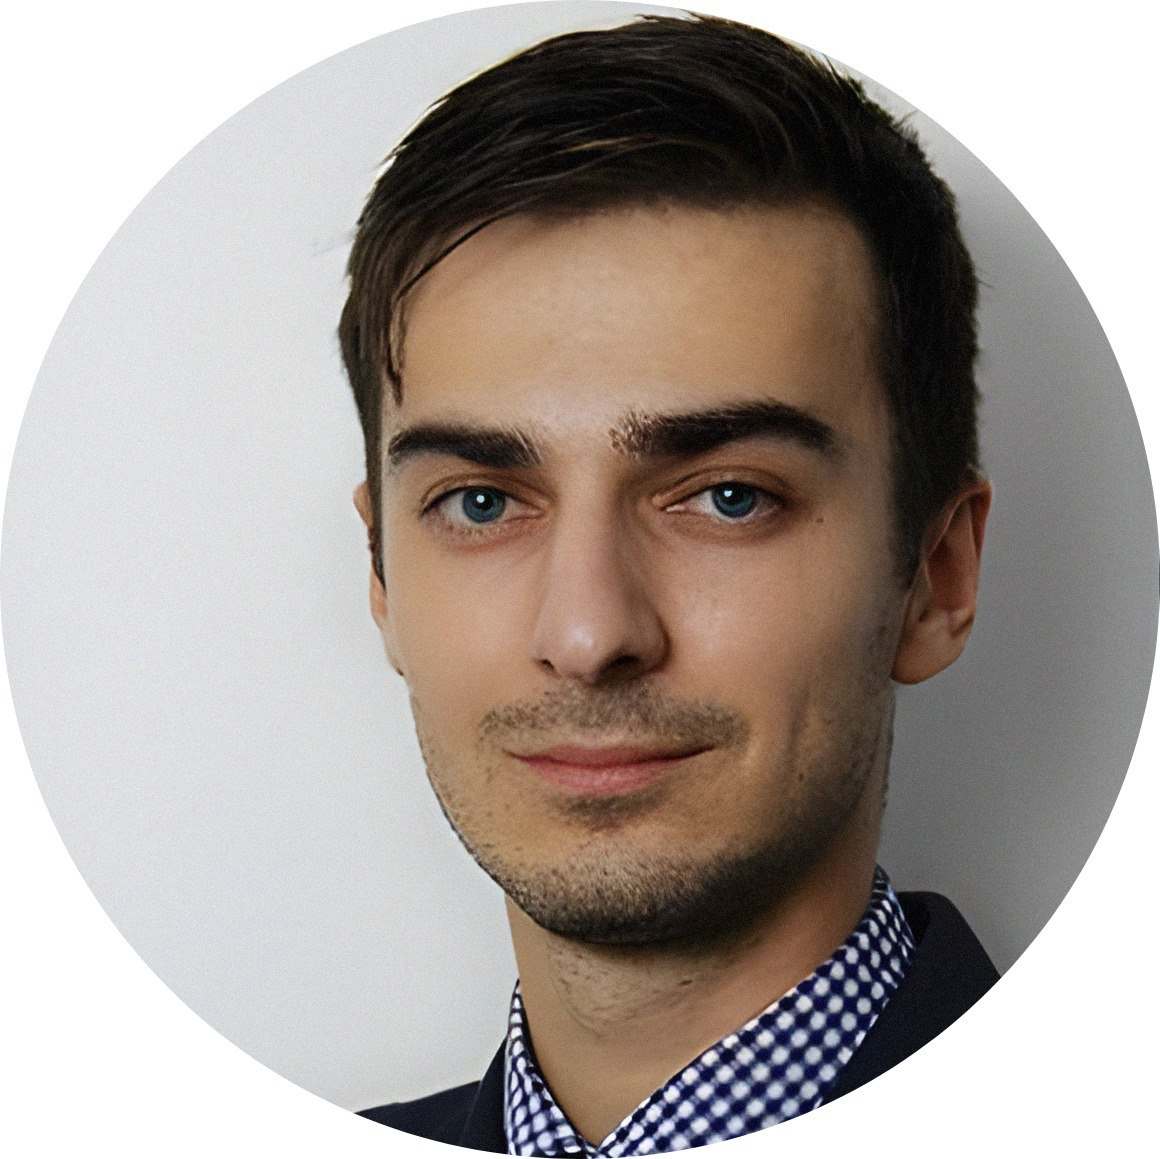
\includegraphics[width=0.95\linewidth]{avatar.png}
\end{minipage}

%\vspace{0.1em}

% Exp ---------------------------------------------------------------------
\begin{minipage}[t]{\textwidth}
\cvsect{Experience}
\begin{entrylist}
  \entry
  {03/2018 -- present}
  {Software Developer}
  {\href{https://dps.de/}{DPS Engineering GmbH, Hamburg}}
  {Development of a European-wide leading system in the area of payment
transactions.\\
 >100 Mio. transactions 24/7 \& >25 big clients banks\\
 Project topics: Domestic and foreign payment transactions, Instant Payments, Clearing \& Settlement, Backoffice, SWIFT, SEPA, MX-Migration, Reporting, etc.\\
 Responsibilities:
  \noseplist{
  % \item \textbf{Guided} the foundation of new team: \textbf{wrote} the team charter and \textbf{defined} team processes.
  % \item \textbf{Acted as Scrum Master.}
  % \item \textbf{Constructed} a new algorithm for identifying similar entities from different sources.
    \item Customer-oriented backend development under time pressure
    \item Analysis, consulting, review, and solution of conceptual design problems
    \item Development, refactoring, maintenance, and optimization under existing legacy
    structures
    \item Support of the test team, test automation
    \item Effort estimation of topics and projects
    }

    \onelinelist{Java, Oracle DB, Git, Docker, Active MQ, JBoss, Jenkins, Kubernetes}
  }
  \entry
  {02/2014 -- 02/2018}
  {Junior Software Engineer}
  {\href{https://envidatec.com/en/}{Envidatec GmbH, Hamburg}}
  {Development of My-JEVis energy monitoring software, which makes it easy and
  cost-effective to keep track of consumption, production data and costs.
  \noseplist{
    % \item \textbf{Guided} the foundation of new team: \textbf{wrote} the team charter and \textbf{defined} team processes.
    % \item \textbf{Acted as Scrum Master.}
    % \item \textbf{Constructed} a new algorithm for identifying similar entities from different sources.
    \item Backend and frontend development in a small agile team
    \item Maintenance, Deployment, Testing, Customer data analysis
    \item Setup of measurement equipment, data collectors and other hardware
    }

    \onelinelist{Java, Spring, MySql, Angular}
  }
\end{entrylist}
\end{minipage}
% EDU -----------------------------------------------------------
\begin{minipage}[t]{0.5\textwidth}
  \cvsect{Education}
\begin{entrylist}
  \otherentry {09/2014 -- 08/2019} {B.A. in Computer Engineering} {\href{https://www.haw-hamburg.de/en/}{Hamburg University of Applied Sciences}} {
    Advanced topics in software engineering, distributed systems, embadded systems and networks.\\
    Thesis: {\href{https://docplayer.org/204520791-Bachelorarbeit-artur-iablokov-kostenanalyse-einer-blockchain-basierten-iot-infrastruktur-mit-ethereum-und-swarm.html}{\emph{Analysis of a blockchain-based IoT infrastructure with Ethereum and Swarm}}}
    %\link{https://docplayer.org/204520791-Bachelorarbeit-artur-iablokov-kostenanalyse-einer-blockchain-basierten-iot-infrastruktur-mit-ethereum-und-swarm.html}{Thesis:}
    %\emph{Analysis of a blockchain-based IoT infrastructure with Ethereum and Swarm}
  }
  \\
  \otherentry {09/2007 -- 06/2012} {B.A. in Management} {\href{https://en.unecon.ru/}{St. Petersburg State University of Economics}} {
    Fundamental theory in mathematics, economics, business administration, information technology and business process management.
  }
\end{entrylist}
\end{minipage}
\hfill
\begin{minipage}[t]{0.45\textwidth}
  \cvsect{Certificates}
  \begin{entrylist}
    %AWS Certified Cloud Practitioner”, 10/2022, Amazon Web Services
    \simpleentry {10/2022} {\href{https://www.credly.com/badges/40fba880-de13-489d-9936-c88cbd59e2d0/}{AWS Certified Cloud Practitioner}} {Amazon Web Services}
    \simpleentry {02/2022} {\href{https://www.udemy.com/certificate/UC-3d1f5088-e87b-4102-8e59-b39df95a5a84/}{React Native - The Practical Guide}} {Udemy}
    \simpleentry {07/2017} {\href{https://app.skillsclub.com/credential/26298-c17cec9e406f32f3ca718dc1ef4aae6d20339ce6fc4964f67f030a661d24137d?locale=de&badge=true}{ISTQB Certified Tester Foundation Level}} {iSQI GmbH}
  \end{entrylist}
\end{minipage}

% Programming languages
\cvsect{Programming \& Tools}

\begin{minipage}[t]{0.35\textwidth} % 50% of the page for the skills bar chart
	\vspace{-\baselineskip} % Required for vertically aligning minipages
	\begin{barchart}{5.5}
		\baritem{Java}{70}
		\baritem{javascript}{50}
		\baritem{SQL}{60}
		\baritem{Spring}{50}
		\baritem{Angular}{40}
	\end{barchart}
\end{minipage}
\hfill
\begin{minipage}[t]{0.6\textwidth}
	\vspace{-\baselineskip} % Required for vertically aligning minipages
	\bubbles{
	4/Docker,
	6/Git,  
    4/nosql,
    5/ethereum, 
	3/k8s,
    4/AWS
	}
\end{minipage}
\vspace{1.5em}

\begin{minipage}[t]{0.25\textwidth}
  \vspace{-\baselineskip}

  \cvsect{Languages}

  \begin{tabular}{ll}
    \textbf{German}   & C1 \\
    \textbf{English} & B2  \\
    \textbf{Russian}    & native
  \end{tabular}
\end{minipage}
\hfill
\begin{minipage}[t]{0.35\textwidth}
  \vspace{-\baselineskip}

  \cvsect{Soft skills}

  \begin{tabular}{ll}
    analysis, logical reasoning,\\prioritizing, constructive feedback,\\responsibility
  \end{tabular}
  %analysis, logical reasoning,\\prioritizing, constructive feedback,\newline responsibility
\end{minipage}
\begin{minipage}[t]{0.35\textwidth}
  \vspace{-\baselineskip}

  \cvsect{Hobbies}
  
  \begin{tabular}{ll}
    surfing, hicking, music concerts,\\podcasts, football, chess
  \end{tabular}
  
\end{minipage}

\end{document}
